\documentclass[tikz]{standalone}

\usepackage{tikz}
\usetikzlibrary{automata}

\begin{document}

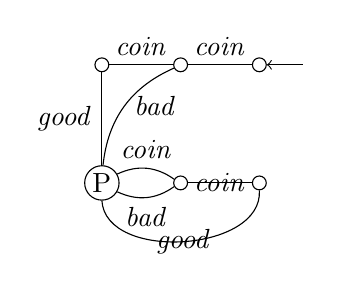
\begin{tikzpicture}
    \tikzstyle{every state}=[
        draw,
        shape=circle,
        inner sep=1pt,
        minimum size=5pt,
        final/.style={double,minimum size=6pt},
        initial text=]

    [auto,->]
    \renewcommand{\a}[1]{\textit{#1}}
    \node[state,initial,initial where=right] (n3) {};
    \node[state, left of=n3] (n4) {};
    \node[state, left of=n4] (n5) {};
    \node[state, below of=n5,yshift=-0.5cm] (n0) {P}; 
    \node[state, right of=n0] (n1) {}; 
    \node[state, right of=n1] (n2) {};
    \path (n3) edge node[above]{\a{coin}} (n4) (n4) edge node[above]{\a{coin}} (n5)
            (n4) edge[bend right] node[right]{\a{bad}} (n0) (n5) edge node[left]{\a{good}} (n0)
            (n0) edge[bend left] node[above]{\a{coin}} (n1) (n1) edge[bend left] node[below]{\a{bad}} (n0)
            (n1) edge node{\a{coin}} (n2) (n2) edge[bend left=90] node{\a{good}} (n0);
\end{tikzpicture}
\end{document}